\section{Обзор предметной области}

\subsection{Встраиваемые функции в Kotlin}

Для начала необходимо дать более полное представление
об использовании встраиваемых функций в Kotlin,
возможностях, которые они предоставляют, а также
ограничениях, которые компилятор накладывает на их использование.

Встраиваемая функция --- любая функция или метод класса в языке Kotlin,
которая помечена аннотацией \texttt{inline}.
Тело такой функции должно быть подставлено компилятором в место вызова.

В качестве примера рассмотрим простейшую функцию, суммирующую два числа:
\begin{listing}[H]
\begin{minted}[frame=lines]{kotlin}
inline fun sum(a: Int, b: Int): Int {
  return a + b
}

val x = sum(1, 2)
\end{minted}
\caption{Пример встраиваемой функции суммирования двух целых чисел}
\end{listing}

Если бы вызов был подставлен программистом вручную, то
значение \texttt{x} было бы инициализировано следующим образом:
\begin{listing}[H]
\begin{minted}[frame=lines]{kotlin}
val x = 1 + 2
\end{minted}
\caption{``Встроенный'' вызов \texttt{sum}}
\end{listing}

Одной из причин добавления встраиваемых функций в Kotlin было
повышение эффективности использования функций высших порядков,
то есть функций, которые принимают в качестве аргументов
другие функции. Вызовы таких функциональных аргументов
встраиваемых функций также подставляются, если такой
аргумент не помечен аннотацией \texttt{noinline}.

В качестве примера рассмотрим функцию \texttt{filter},
которая принимает на вход список и предикат, а возвращает
новый список, содержащий только те значения из
первого списка, которые удовлетворяют предикату:
\begin{listing}[H]
\begin{minted}[frame=lines]{kotlin}
inline fun filter<T>(list: T, predicate: (T)->Boolean): List<T> {
  val filtered = arrayListOf<T>()

  for (x in list) {
    if (predicate(x)) {
      filtered.add(x)
    }
  }

  return filtered
}
\end{minted}
\caption{Пример функции высшего порядка filter}
\label{lst:filter-example}
\end{listing}

Чаще всего в качестве аргумента такой функции используются анонимные
функции, для каждой из которых в случае платформы JVM необходимо
сгенерировать новый класс (при этом вызов предиката будет виртуальным).
Однако в случае встраиваемых функций можно подставить вызов
и функции \texttt{filter}, и её аргумента \texttt{predicate}.
Таким образом, использование функций высших порядков не
несёт каких-либо дополнительных накладных расходов (по сравнению
с написанием цикла руками в случае с \texttt{filter}).

Помимо операций над коллекциями функции высших порядков
могут использоваться для создания доменно-специфичных
языков. В качестве примера рассмотрим использование
функций для описания \texttt{html}-разметки:
\begin{listing}[H]
\begin{minted}[frame=lines]{kotlin}
inline fun tag(name: String, inner: ()->String): String =
  "<$name>" + inner() + "</$name>"
inline fun html(html: ()->String): String = tag("html", html)
inline fun body(body: ()->String): String = tag("body", body)
inline fun h1(h1: ()->String): String = tag("h1", h1)

fun main(args: Array<String>) {
    val simpleHtml =
        html {
            body {
                h1 { "Simple HTML builders!" }
            }
        }

    println(simpleHtml)
}
\end{minted}
\caption{Пример простого доменно-специфичного языка для описания HTML-разметки}
\end{listing}

В этом примере блоки, которые следуют за вызовами функций
\texttt{html}, \texttt{body}, \texttt{h1},
являются всего лишь анонимными функциями.
Такой код выглядит лаконично, однако за счёт генерации большого
количества вложенных друг в друга функций, несёт дополнительные
накладные расходы. Встраивание позволит сократить
число сгенерированных классов для JVM.

В случае JavaScript встраивание небольших функций может
уменьшить размер кода. Однако в случае больших функций
встраивание увеличит размер кода, что может
отрицательно сказываться на времени передачи по сети, а также
на времени работы синктаксического анализатора.

Необходимость встраивания с точки зрения влияния
на производительность JavaScript кода неоднозначна.
С одной стороны, все многие современные среды исполнения
JavaScript (к примеру V8 в браузере Google Chrome)
используют Just-In-Time (JIT) компиляцию, когда горячие
участки кода компилируются и оптимизируются во
время исполнения. Обычно JIT-компиляторы
сами умеют производить встраивание, однако
существуют случае, когда этого не происходит:
\begin{itemize}
  \item Функции, которые вызываются недостаточно большое число раз (зависит
  от конкретного компилятора).
  \item Мегаморфные функции. Современные JIT-компиляторы смотрят
  на то, какие типы функция принимает на вход. В данном случае типы
  определяются эвристически из-за динамической природы JavaScript
  (упрощённо можно считать, что разные типы имеют объекты разной структуры).
  Когда компилятор видит, что функция часто вызывается с разными типами,
  он считает её мегаморфной и перестаёт оптимизировать.
  Теоретически шаблонные функции высших порядков могут попадать
  под это определение.

\end{itemize}

\subsection{Нелокальные возвраты}

При встраивании возможно использование внутри анонимных функций
нелокальных возвратов~\cite{NONLOCAL_RETURN}. Проще всего рассмотреть эту возможность на следующем примере:
\begin{listing}[H]
\begin{minted}[frame=lines]{kotlin}
inline fun forEach<T>(list: List<T>, block: (T)->Unit): Unit {
  for (x in list) {
    block(x)
  }
}

fun main(args: Array<String>) {
  // будет напечатано 3 2 1
  forEach(listOf(3, 2, 1, 0)) { int ->
    if (int == 0) return@forEach
    print("$int ")
  }
}
\end{minted}
\caption{Пример использования нелокального возврата}
\end{listing}

В данном примере из анонимной функции, которая передаётся в качестве
аргумента \texttt{forEach}, производится возврат сразу из вызова
функции \texttt{forEach}. Также возможно сделать возврат из функции \texttt{main}.
Без использования встраиваемых функций такую функциональность
реализовать невозможно. В будущих версиях языка
должна появиться поддержка нелокальных
\texttt{break} и \texttt{continue}.
На данный момент поддержка нелокальных возвратов реализована только
для платформы JVM.

\subsection{Ограничения встраиваемых функций}

Компилятор Kotlin накладывает некоторые ограничения на встраиваемые
функции:
\begin{itemize}
  \item Встраиваемая функция не может быть виртуальной. Действительно,
  в общем случае подстановка таких функций
  на этапе компиляции невозможна.
  \item Встраиваемая функция не может быть рекурсивной. Очевидно, что
  процесс подстановки рекурсивной функции будет продолжаться,
  пока не кончится стек.
  \item Публично-доступная встраиваемая функция не может захватывать
  непубличные функции и значения.
  Публично-доступной считается функция, которая объявлена с модификатором
  \texttt{public} и, если она является членом какого-либо
  класса или объекта, то он также должен быть публично-доступным.
  \item Если функциональный аргумент
  встраиваемой функции используется любым способом, кроме
  вызова и передачи другой встраиваемой функции, то такой аргумент должен быть помечен
  аннотацией \texttt{noinline} (вызовы такого аргумента не будут
  встроены). Примером такого использования может служить запись
  ссылки на функцию в переменную.
  \item Если функциональный аргумент встраиваемой функции захватывается
  локальным объектом, то такой аргумент должен быть помечен аннотацией
\\  \texttt{inlineOptions(InlineOption.ONLY\_LOCAL\_RETURN)} (такой аргумент
  не должен содержать нелокальных возвратов).
  \item Конструктор не может быть встраиваемой функцией.
\end{itemize}

Следующие ограничения носят временный характер и могут быть сняты
в будущих версиях языка:
\begin{itemize}
  \item Встраиваемая функция не может содержать объявления функций и классов.
  \item Функциональный аргумент встраиваемой функции не может
    иметь значение по умолчанию (либо должен быть помечен аннотацией
    \texttt{noinline}).
\end{itemize}

При нарушении вышеперечисленных ограничений компилятор сообщит об ошибке.

Отдельно стоит упомянуть, что вызовы функциональных аргументов встраиваемой функции, помеченные
ключевым словом \texttt{vararg} (количество соответствующих
аргументов не фиксировано), не могут быть встроены (однако
такое использование не считается ошибкой компиляции).

\subsection{Процесс компиляции Kotlin}

\begin{figure}[H]
\begin{tikzpicture}[%
  x=1.25cm,y=2cm,
  font=\footnotesize,
  imageNode/.style={inner sep=0pt},
  textAbove/.style={align=center, yshift=36mm},
  textBelow/.style={align=center, yshift=10.5mm}
  ]

\newcommand\fileImage[0]{
\includegraphics[width=.10\textwidth]{images/icon-file}}
\newcommand\metadataImage[0]{
\includegraphics[width=.12\textwidth]{images/metadata}}
\newcommand\astImage[0]{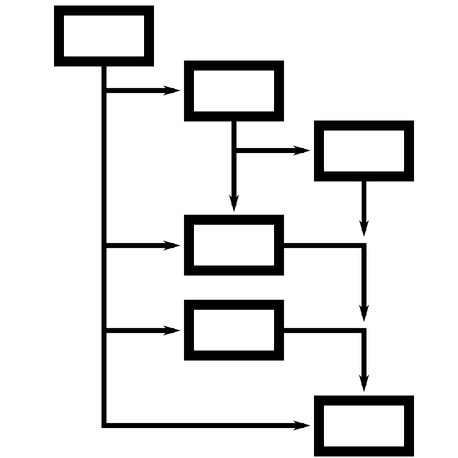
\includegraphics[width=.12\textwidth]{images/ast}}

\newcommand\drawFile[4][]{%
	\node[imageNode, #1] (#4) {\fileImage};
	\node[textAbove, below=of #4] {#2.#3};
}
\newcommand\ktFile[2][]{\drawFile[#1]{#2}{kt}{#2}}
\newcommand\jsFile[2][]{\drawFile[#1]{#2}{js}{#2}}
\newcommand\metaJsFile[2][]{\drawFile[#1]{#2}{meta.js}{meta#2}}

\newcommand\drawFileBelow[4][]{%
	\node[imageNode, #1] (#4) {\fileImage};
	\node[textBelow, below=of #4] {#2.#3};
}
\newcommand\ktFileBelow[2][]{\drawFileBelow[#1]{#2}{kt}{#2}}
\newcommand\jsFileBelow[2][]{\drawFileBelow[#1]{#2}{js}{#2}}
\newcommand\metaJsFileBelow[2][]{\drawFileBelow[#1]{#2}{meta.js}{meta#2}}

\newcommand\drawBoxWithOptions[4]{%
\begin{scope}[on background layer]
	\node[rounded corners, draw=black, very thick, dashed, fill=lightgray!10,
    	fit=#1,
    	label={[yshift=0mm]#2},
    	#4
    ] (#3) {};
\end{scope}
}

\newcommand\drawBox[3]{\drawBoxWithOptions{#1}{#2}{#3}{inner ysep=5mm, inner xsep=3mm}}

\ktFile{main}
\ktFile[right=of main, xshift=-5mm]{util}
\drawBox{(main)(util)}{Программа}{ktFiles}

\metaJsFile[right=of ktFiles, xshift=5mm]{lib}
\jsFile[right=of metalib, xshift=-5mm]{lib}
\drawBox{(lib)(metalib)}{Библиотека}{jsFiles}

\node[imageNode, below=of metalib, yshift=-15mm] (libraryMetadata) {\metadataImage};
\node[xshift=10mm, left=of libraryMetadata,align=center] {Метаданные\\библиотеки};

\node[imageNode, below=of ktFiles, yshift=-10mm] (ktAst) {\astImage};
\node[xshift=10mm, left=of ktAst] (ktAstText) {Kotlin AST};

\node[imageNode, below=of ktAst,yshift=-10mm] (programMetadata) {\metadataImage};
\node[xshift=10mm, left=of programMetadata,align=center] (programMetadataText) {Метаданные\\программы};

\drawBox{(programMetadata)(programMetadataText)(ktAstText)(libraryMetadata)}{}{codegenInput}

\node[imageNode, right=of codegenInput, xshift=21mm, yshift=20mm] (jsAst) {\astImage};
\node[above=of jsAst, yshift=-8mm] (jsAstText) {JavaScript AST};

\metaJsFileBelow[right=of programMetadata,xshift=50mm]{program}
\jsFileBelow[right=of metaprogram, xshift=-5mm]{program}
\drawBoxWithOptions{(program)(metaprogram)}{}{output}{inner sep=5mm}

% Arrows
\tikzstyle{fatArrow}=[line width=1mm,-triangle 90,postaction={draw, line width=3mm, shorten >=1.4mm, -}]
\draw [fatArrow](ktFiles.south) -- node[anchor=west,align=center, yshift=2mm] {~(1) Синтаксический\\анализ} (ktAst.north);
\draw [fatArrow](metalib.south) -- node[anchor=west,align=center, yshift=1mm] {~(2) Десериализация} (libraryMetadata.north);
\draw [fatArrow](ktAst.south) -- node[anchor=west,align=center] {~(3) Семантический\\анализ} (programMetadata.north);
\draw [fatArrow]($(codegenInput.east) + (0,1)$) -- node[anchor=north,align=center,yshift=-2mm,xshift=0mm] {(4) Трансляция} (jsAst.west);
\draw [fatArrow](jsAst.south) -- node[anchor=west,align=center,yshift=3mm] {~(5) Сериализция} (program.north);
\draw [fatArrow](programMetadata.east) -- node[anchor=north,align=center,yshift=-2mm,xshift=-10mm] {~(6) Сериализция} (metaprogram.west);

\end{tikzpicture}

\caption{Схема процесса компиляции Kotlin в JavaScript без встраивания функций}
\label{fig:compilation1}
\end{figure}

Перед описанием процесса компиляции стоит пояснить,
что является результатом компиляции программы на языке Kotlin:
\begin{itemize}
  \item Файл с расширением \texttt{.js}, который содержит
  определения функций и классов на языке JavaScript.
  \item Опционально (передав ключ компиляции \texttt{-meta-info}),
  пользователь может сгенерировать файл с расширением
  \texttt{.meta.js}, который содержит сериализованные метаданные,
  то есть информацию о сигнатурах функций и классов,
  полученную в результате семантического анализа.
  Такой файл позволяет не проводить семантический и синтаксический
  анализ библиотеки повторно при компиляции программ,
  использующих её. Этот же механизм используется
  при раздельной компиляции модулей в плагине Kotlin для
  Intellij IDEA IDE.
\end{itemize}

Процесс компиляции программы на языке Kotlin без поддержки встраиваемых
функций схематично изображён на рис. \ref{fig:compilation1}. Опишем
шаги компиляции подробнее:
\begin{enumerate}
  \item Производится синтаксический анализ исходных кодов программы.
  Результатом является абстрактное синтаксическое дерево.
  Это дерево содержит только структуру кода. Однако
  тот факт, что код синтаксически корректен не означает,
  что в нём нет ошибок. К примеру в коде может
  присутствовать вызов несуществующей функции.
  Также на этом этапе не хватает метаданных (в частности
  неизвестно, какой функции соответствует тот или иной вызов).
  \item Производится десериализация библиотек.
  Как уже было сказано ранее, библиотеки имеют расширение
  \texttt{.meta.js} и представляют собой валидный
  JavaScript код, содержащий метаданные,
  сериализованные в строку.
  \item На основе Kotlin AST и метаданных библиотек
  производится семантический анализ программы.
  Результатом этого этапа являются метаданные программы.
  \item На основе Kotlin AST и метаданных программы
  производится трансляция в JavaScript AST (синтаксического
  дерева, которое описывает структуру конечного кода на языке
  JavaScript).
  \item JavaScript AST сериализуется в файл.
  \item Метаданные программы сериализуются в файл.
\end{enumerate}

Скомпилированные библиотеки могут содержать
встраиваемые функции. Так как библиотечные
файлы не содержат исходных кодов на языке Kotlin,
то встраивание необходимо производить
после трансляции Kotlin AST в JavaScript AST.

Теперь, когда дано определение встраиваемых функций в
Kotlin и описан процесс компиляции, можно
сформулировать цель и задачи работы.

\subsection{Цель и задачи}

Целью данной работы является поддержка встраиваемых
функций при компиляции Kotlin в JavaScript.

Для достижения поставленной цели необходимо решить
следующие задачи:
\begin{enumerate}
  \item Провести исследование существующих решений.
  Как уже было сказано во введении,
  компиляция в JavaScript стала весьма популярной
  в последнее время, а подстановка функций
  является одной из основных оптимизаций в компиляторах.
  Поэтому разумно изучить уже существующие решения,
  исследовать возможность переиспользования кода.
  \item Обеспечить работу встраивания без поддержки
  встраивания из библиотек. При этом,
  встраивание должно производится на основе JavaScript AST.
  \item Обеспечить встраивание функций из библиотек. Для этого
  необходимо решить задачи нахождения скомпилированных
  функций и синтаксического анализа JavaScript кода.
  \item Проанализировать влияние подстановки функций
  на производительность JavaScript кода.
\end{enumerate}

\subsection{Существующие решения}

\subsubsection{Google Web Toolkit}

Google Web Toolkit (GWT) -- Java-фреймворк, который позволяет
создавать веб-приложения на Java. Включает в себя компилятор
из Java в JavaScript. Компилятор осуществляет некоторые
оптимизации над JavaScript деревом, в том числе подстановку
функций.

Классы JavaScript AST, используемые в Kotlin, были когда-то
взяты из GWT (исходные коды проекта открыты), хотя
и притерпели некоторые изменения. Поэтому
GWT привлекателен с точки зрения исследования
возможности переиспользования реализации встраивания.

Процесс встраивания происходит следующим образом:
\begin{enumerate}
  \item Параметры функции заменяются на аргументы вызова.
  Если аргументы могут содержать побочные эффекты, и
  некоторые из соответствующих параметров не используются,
  либо могут использоваться
  в другом порядке, то встраивание не производится.
  \item Декларации (\texttt{var} утверждения) локальных
  переменных добавляются в начало вызывающей функции. Если
  декларация переменной была инициализирована, то присваивание значения
  не переносится. То есть в утверждении \texttt{var x = 10;}
  декларация \texttt{var x;} будет перенесена, а инициализация
  \texttt{x = 10;} останется на месте.
  \item Тело функции переписывается в виде выражения через запятую.
  Семантика бинарного оператора запятая следующая: сначала выполняется левая
  часть выражения, затем правая, в качестве результата возвращается
  значение, полученное в результате вычисления правого подвыражения.
  К такому виду можно привести очень ограниченное число функций.
  К примеру, ни один цикл в JavaScript не может быть частью выражения.
  \item Вызов заменяется на получившееся выражение.
\end{enumerate}

Как видно из описания процесса, такой подход работает
лишь в некоторых случаях.

\subsubsection{Closure Compiler}

Closure Compiler (CC) -- минификатор JavaScript. Также может
рассматриваться в качестве продвинутого оптимизирующего компилятора
JavaScript в JavaScript, хотя увеличение производительности
не является главной целью проекта.

На функцию, которая может быть встроена накладывается
существенно меньше ограничений, чем в GWT:
\begin{enumerate}
  \item Функция не должна быть рекурсивной.
  \item Функция не содержит объявлений других функций.
  \item Функция вызывается один раз или размер тела функции
  меньше, чем всё её определение (минимальное определение
  функции в JavaScript: ``\mintinline{javascript}{function(){}}'').
  \item Имя функции не используется в других контекстах, кроме вызова
  (то есть сслыка на функцию не может быть сохранена в переменную).
\end{enumerate}

Таким образом, функциональность Closure Compiler позволяет
встраивать большую часть функций, которые могут быть встраиваемыми
в Kotlin. Однако использование CC для подстановки функций в Kotlin
затруднительна по следующим причинам:
\begin{itemize}
  \item Невозможно форсировать встраивание, если использовать
  CC, как библиотеку. Таким образом без копирования проекта
  и внесения изменений в код гарантировать встраивание функций
  невозможно.
  \item Использование на уровне исходных кодов также затруднительно
  из-за другого формата AST. Решение с конвертацией JS AST Kotlin в JS AST Closure
  Compiler возможно, однако такое решение может быть довольно хрупким
   (например при изменении структуры генерируемого кода). К тому же
   обеспечение дополнительной функциональности встраиваемых функций в Kotlin
   (нелокальные возвраты) потребовало бы дополнительных
   изменений в коде Closure Compiler, либо обратной конвертации AST.
\end{itemize}

Из-за перечисленных выше причин было принято решение о
написании своей реализации встраивания.
